\documentclass[12pt,aspectratio=169,xcolor=dvipsnames]{beamer}
\usetheme{SimplePlus}
\usepackage{booktabs}
\usepackage{tikz,subcaption}
\usepackage{pgfplots}
\usepackage{mathtools}

\newcommand{\R}{\mathbb{R}}
\newcommand{\N}{\mathbb{N}}

\title[short title]{Clase 15 Análisis de señales}
\subtitle{}
\author[NA Barnafi] {Nicolás Alejandro Barnafi Wittwer}
\institute[UC|CMM] 
{
    Pontificia Universidad Católica de Chile \\
    Centro de Modelamiento Matemático
}

\titlegraphic{
    \vspace{-1.8cm}
    \begin{flushright}
      
\includegraphics[height=2.5cm]{../images/puc.png} 
    \end{flushright}
}

\date{05/05/2025}
%\setbeamercovered{transparent}

\begin{document}
%%%%%%%%%%%%%%%%%%%%%%%%%%%%%%%%%%%%%%%%%%%%%%%%%%%%%%%
\begin{frame}
    \maketitle
\end{frame}
%%%%%%%%%%%%%%%%%%%%%%%%%%%%%%%%%%%%%%%%%%%%%%%%%%%%%%%
\begin{frame}{Clase de hoy}
    \begin{itemize}
        \item Señales
        \item Espacios de Hilbert y sus propiedades
        \item Ejemplos
    \end{itemize}

    \vspace{1cm}
    \newref{Curso análisis de Fourier}
\end{frame}
%%%%%%%%%%%%%%%%%%%%%%%%%%%%%%%%%%%%%%%%%%%%%%%%%%%%%%%
\begin{frame}{Señales}
    \begin{center}
        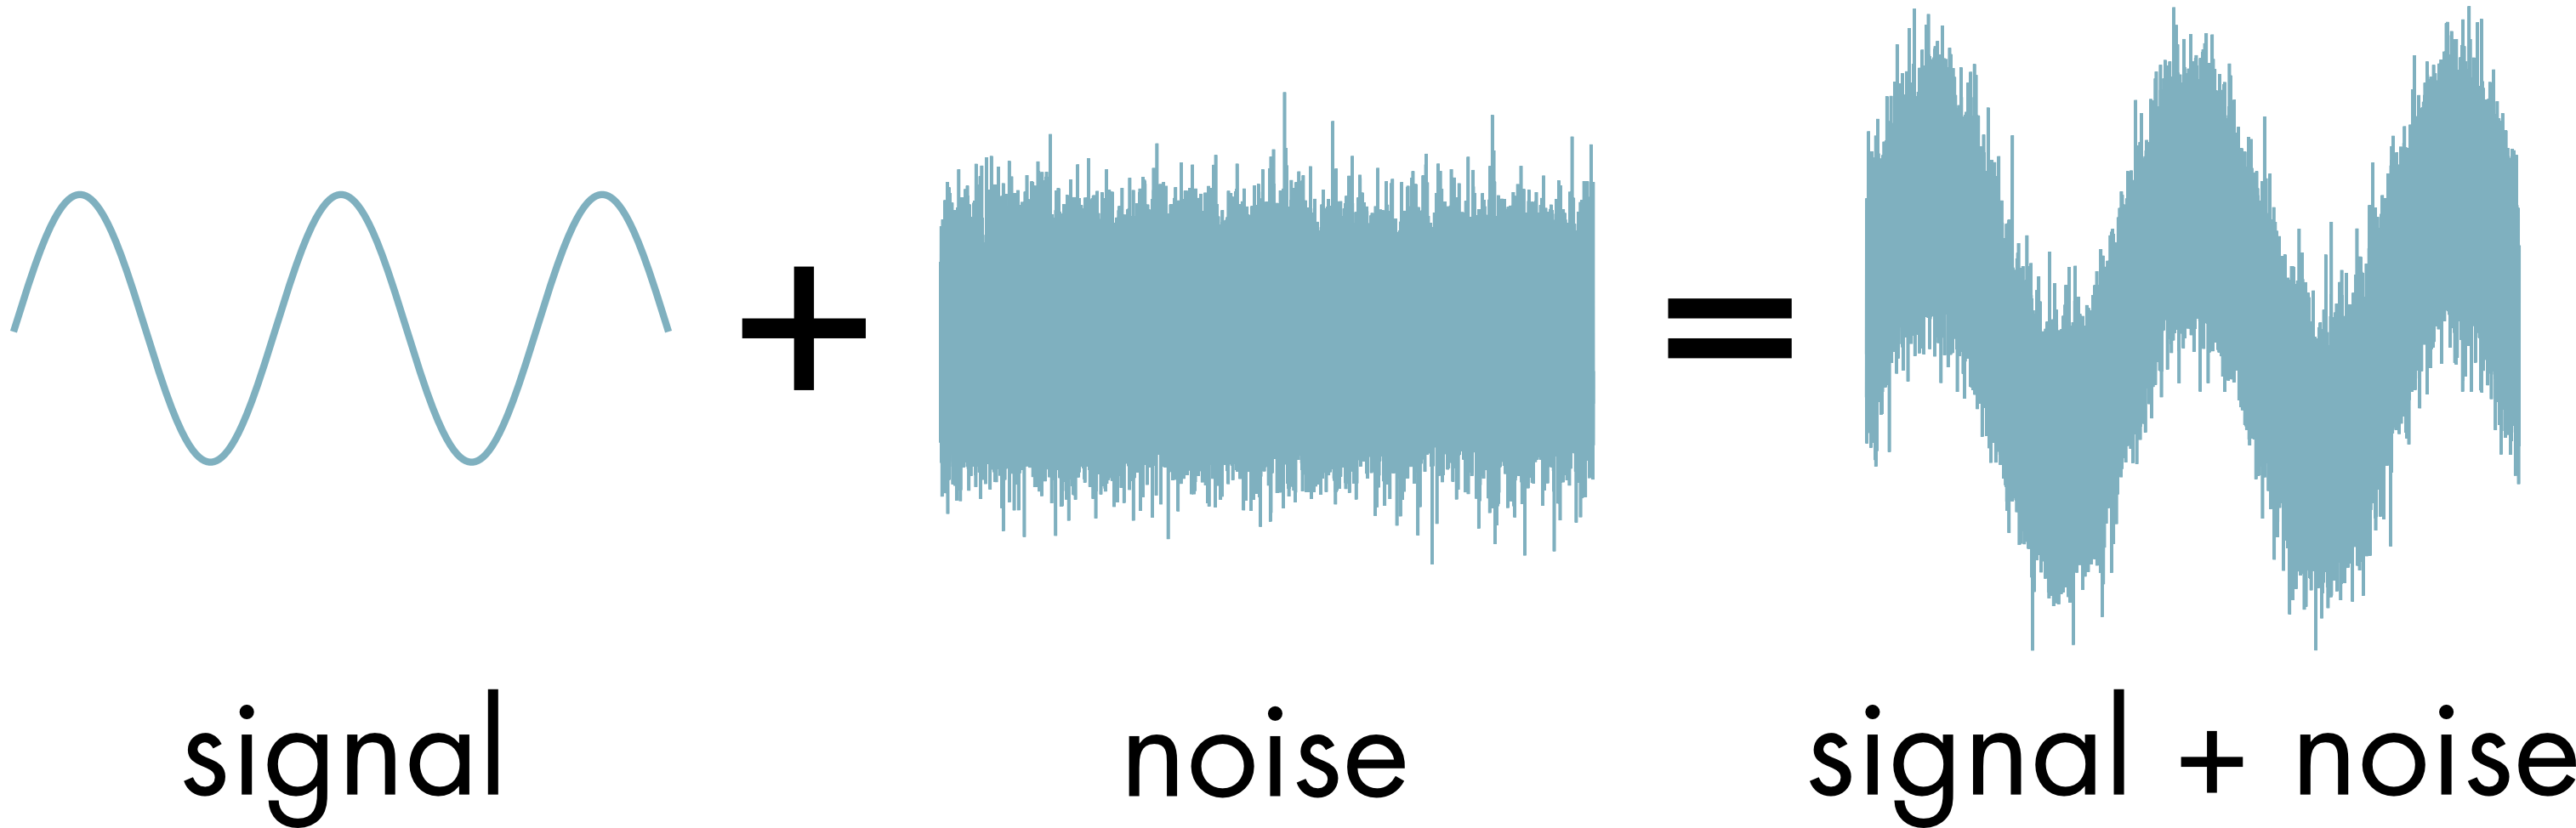
\includegraphics[width=\textwidth]{../images/s2n.png}
    \end{center}
    \alertGreen{Aspectos de modelamiento: superposición, filtro, etc}
\end{frame}
%%%%%%%%%%%%%%%%%%%%%%%%%%%%%%%%%%%%%%%%%%%%%%%%%%%%%%%
\begin{frame}{En el lenguaje de lo que conocemos}
    \begin{itemize}
        \item<+-> Una señal es una función $\to$ un punto de un espacio funcional
            $$ f(x) = \sin x $$
        \item<+-> Las señales se pueden superponer (suma!)
            $$ f_1(x)=\sin x, \quad f_2(x) = \cos x \quad \Rightarrow (f_1+f_2)(x) = \sin x + \cos x$$
        \item<+-> Las señales se pueden modular (producto por escalar!)
            $$ f(x) = \sin x \quad \Rightarrow (\alpha f)(x) = \alpha \sin x $$
    \end{itemize}
\end{frame}
%%%%%%%%%%%%%%%%%%%%%%%%%%%%%%%%%%%%%%%%%%%%%%%%%%%%%%%
\begin{frame}\frametitle{Intuición}
    \begin{itemize}
        \item Espacios de funciones 'regulares'
        \item Funciones trigonométricas son una base
            $$ \begin{bmatrix} 1 \\ 2 \end{bmatrix} = 1 \, \begin{bmatrix} 1 \\ 0\end{bmatrix} + 2 \begin{bmatrix} 0 \\ 1\end{bmatrix} $$
            O sea que podríamos escribir
            $$ f(x) = a_0 + \sum_k \alpha_k \sin (k\pi x) + \beta_k \cos(k \pi x) $$
    \end{itemize}

\end{frame}
%%%%%%%%%%%%%%%%%%%%%%%%%%%%%%%%%%%%%%%%%%%%%%%%%%%%%%%
\begin{frame}
    \begin{figure}
        \begin{subfigure}{0.3\textwidth}
            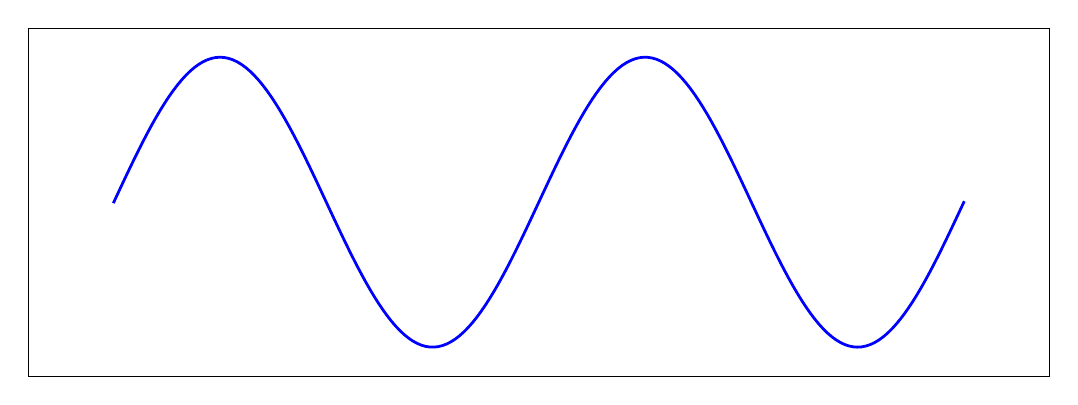
\begin{tikzpicture}
                \begin{axis}[width=1.2\textwidth,height=6cm,ticks=none]
                    \addplot[domain=-6.29:6.29,
                            samples=200,
                            color=blue,
                            line width=1pt]{sin(deg(x))};
                \end{axis}
            \end{tikzpicture}
            \caption*{$sin(x)$}
        \end{subfigure}
        \begin{subfigure}{0.3\textwidth}
            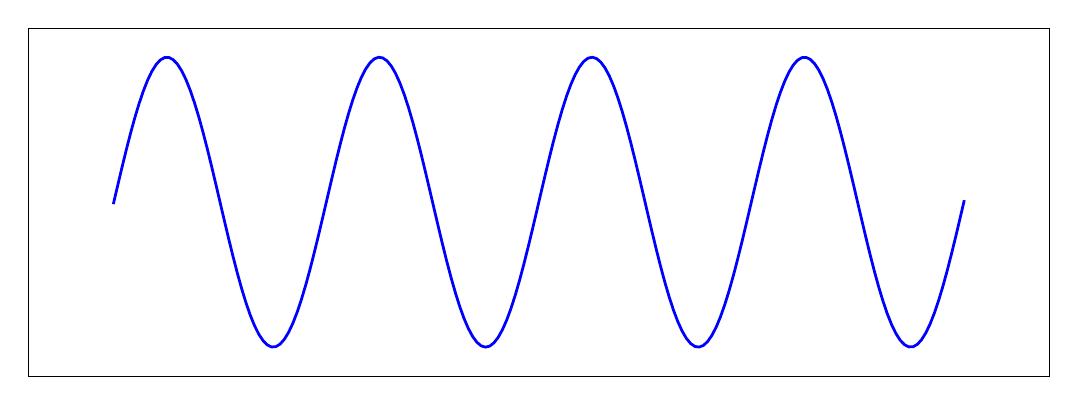
\begin{tikzpicture}
                \begin{axis}[width=1.2\textwidth,height=6cm,ticks=none]
                    \addplot[domain=-6.29:6.29,
                            samples=200,
                            color=blue,
                            line width=1pt]{sin(deg(2*x))};
                \end{axis}
            \end{tikzpicture}
            \caption*{$sin(2x)$}
        \end{subfigure}
        \begin{subfigure}{0.3\textwidth}
            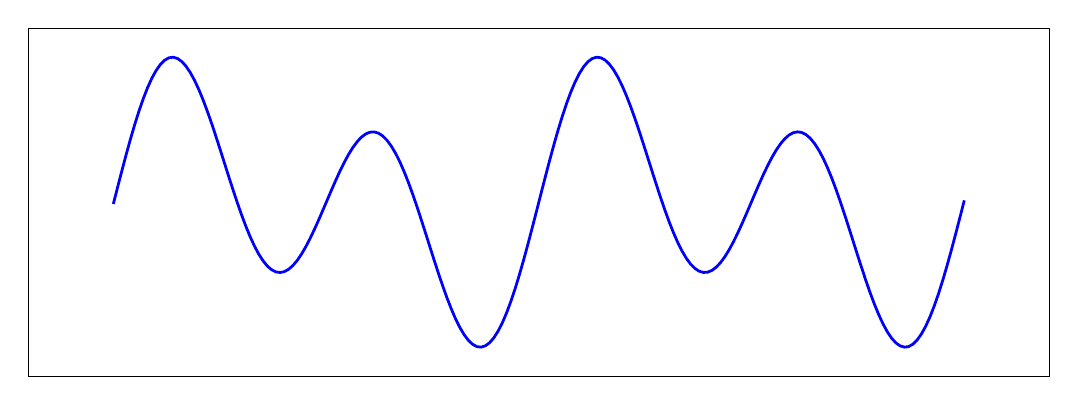
\begin{tikzpicture}
                \begin{axis}[width=1.2\textwidth,height=6cm,xmajorticks=false,ymajorticks=false]
                    \addplot[domain=-6.29:6.29,
                            samples=200,
                            color=blue,
                            line width=1pt]{2*sin(deg(2*x)) + sin(deg(x))};
                \end{axis}
            \end{tikzpicture}
            \caption*{$2\, sin(x) + sin(2x)$}
        \end{subfigure}
    \caption*{Combinación lineal de elementos en el espacio}
    \end{figure}
\end{frame}
%%%%%%%%%%%%%%%%%%%%%%%%%%%%%%%%%%%%%%%%%%%%%%%%%%%%%%%
\begin{frame}{Independencia lineal}
    Combinaciones lineales permiten establecer dependencia entre funciones.
    \begin{block}{Independencia lineal}
        Un conjunto de funciones $f_1, \hdots, f_N$ es linealmente independiente si
          $$\sum_{i=1}^N \alpha_i f_i = 0 $$
          implica
          $$ \alpha_i = 0$$
    \end{block}
    \begin{itemize}
        \item<+-> Ej: $\sin$  y $\cos$ son linealmente independientes
        \item<+-> Identidades trigonométricas son \emph{dependencia lineal}
    \end{itemize}
    \idea{Interpretar identidad $\cos 2\theta = 2\cos^2\theta-1$ como dependencia lineal de funciones }
\end{frame}
%%%%%%%%%%%%%%%%%%%%%%%%%%%%%%%%%%%%%%%%%%%%%%%%%%%%%%%
\begin{frame}{Espacios de Hilbert}
    \begin{block}{Espacio de Hilbert}
        Espacio vectorial normado \textcolor{gray}{(completo)}\footnote{Análisis real} $H$ con un producto interno $(\cdot,\cdot):H\times H\to \R$ tal que
        \begin{itemize}
            \item Simétrico: $(x,y) = (y,x)$
            \item Lineal en primer argumento: $(ax + by, z) = a(x,z) + b(y,z)$
            \item Definido positivo: $(x,x)\geq 0$, es 0 solo si $x=0$. 
        \end{itemize}
        Notar que el producto interno define una norma $|x| = \sqrt{(x,x)}$. 
    \end{block}
    \idea{Verificar que producto interno de vectores $x\cdot y=\sum x_iy_i$ las cumple}
\end{frame}
%%%%%%%%%%%%%%%%%%%%%%%%%%%%%%%%%%%%%%%%%%%%%%%%%%%%%%%
\begin{frame}{Proyección y Ortogonalización}
    Veamos primero en $\R^2$. Sean $x,y$ vectores. 
    \begin{itemize}
        \item Normalización:
            $$ \hat y = \frac{y}{|y|} $$
        \item Ángulo entre vectores
            $$ x\cdot y = |x||y|\angle(x,y) $$
        \item Proyección de $x$ en dirección $y$.
            $$P_y(x) = (x, \hat y)\hat y = \left(x, \frac{y}{|y|}\right)\frac{y}{|y|} = \hat y\hat y^T x $$
        \item Ortogonalización de $x$ con respecto a $y$
            $$ x^\perp = x - P_y(x) = (\mathbf I - \hat y \hat y^T) x $$
    \end{itemize}
    \idea{Qué relación tiene esto con la factorización QR?}
\end{frame}
%%%%%%%%%%%%%%%%%%%%%%%%%%%%%%%%%%%%%%%%%%%%%%%%%%%%%%%
\begin{frame}{Construcción de producto interno en dim infinita}
    Consideramos norma $L^2(0,1)$: $\| f \|^2 = \int_0^1 f^2(x)\,dx$
    \begin{align*}
        \| u + v \|^2 &= \int_0^1(u(x) + v(x))^2\,dx \\
                    &= \int_0^1u^2(x)\,dx + 2\int_0^1u(x)v(x)\,dx + \int_0^1v^2(x)\,dx \\
                    &= \| u \|^2 + 2\int_0^1u(x)v(x)\,dx  + \| v \|^2. 
    \end{align*}
    Definimos $(u,v) = \int_0^1uv\,dx$. 
\end{frame}
%%%%%%%%%%%%%%%%%%%%%%%%%%%%%%%%%%%%%%%%%%%%%%%%%%%%%%%
\begin{frame}{Relación con Teo coseno}
    \begin{center}
        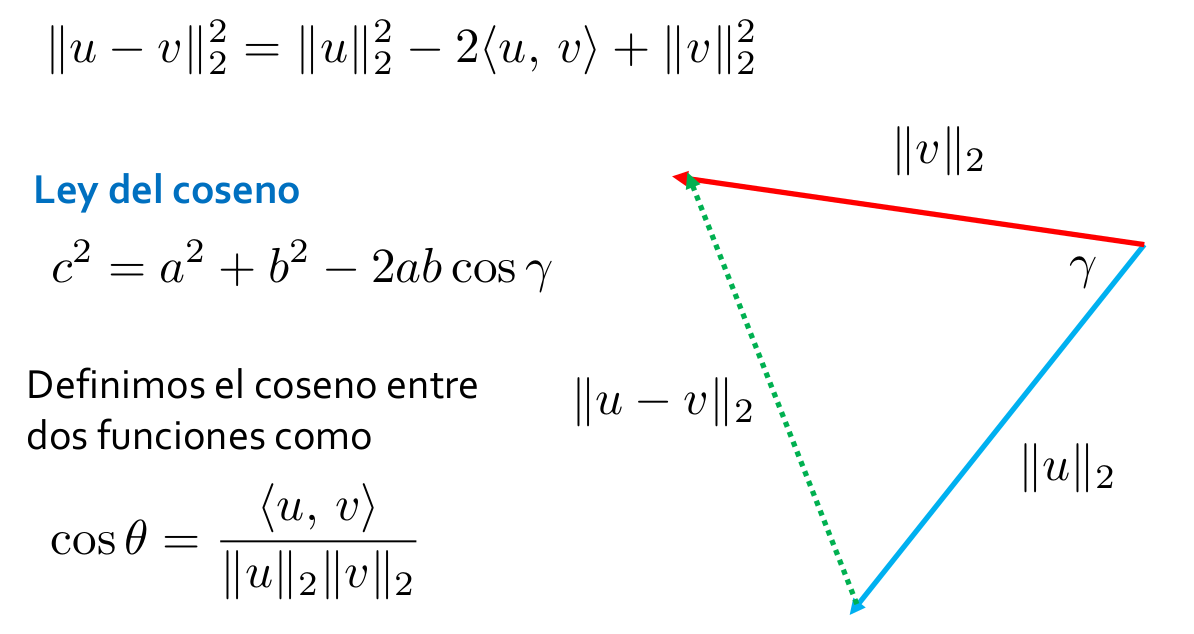
\includegraphics[width=0.7\textwidth]{../images/teorema-coseno.png}\footnote{C Sing-Long}
    \end{center}
    \alert{Esto \emph{define} al producto interno vectorial!}
\end{frame}
%%%%%%%%%%%%%%%%%%%%%%%%%%%%%%%%%%%%%%%%%%%%%%%%%%%%%%%
\begin{frame}{En dimensión infinita}
    Un producto interno entre funciones $f,g:(-1,1)\to \R$ (cuando esté bien definido) es
    $$ (f,g) = \int_{-1}^1 fg\,dx.$$
    Se le llama \emph{producto $L^2((-1,1),\R)$}. Con esto podemos: 
        \begin{itemize}
            \item Normalizar
            \item Proyectar
            \item Ortogonalizar
        \end{itemize}
        \idea{Calcular proyección de $f(x)=x$ en función $g(x)=1$}
        \idea{Demostrar que $\sin(k_1\pi x)$ y $\cos(k_2\pi x)$ son ortogonales}
\end{frame}
%%%%%%%%%%%%%%%%%%%%%%%%%%%%%%%%%%%%%%%%%%%%%%%%%%%%%%%
\begin{frame}{Ejemplo}
    Encontrar coeficientes $\alpha_i$,$\beta_i$ tales que
        $$ f(x) = \begin{cases} -1 & x \in (-1,0) \\ 1 & x \in (0,1) \end{cases} $$
    se puede escribir como
        $$ f(x) = a_0 + \sum_k \alpha_k \sin(k\pi x) + \beta_k\cos(k\pi x) $$
    Será útil recordar que $\sin(k_1\pi x)$ y $\cos(k_2\pi x)$ son ortogonales.
\end{frame}
%%%%%%%%%%%%%%%%%%%%%%%%%%%%%%%%%%%%%%%%%%%%%%%%%%%%%%%
\begin{frame}
    \maketitle
\end{frame}
%%%%%%%%%%%%%%%%%%%%%%%%%%%%%%%%%%%%%%%%%%%%%%%%%%%%%%%
\end{document}
